\documentclass[13pt]{jarticle}


\title{競技プログラミングアドベントカレンダー2017\\
  Day2 : ”花火”に対するシンプルな解法}
\author{tokoharu}

\date {2017.12.02}

\usepackage{amsthm}
\usepackage{algorithm}
\usepackage{algorithmic}
\usepackage{ascmac}
\usepackage{amsmath}
\usepackage{courier}
%\usepackage{eqnarray}
\usepackage[dvipdfmx]{graphicx}
\usepackage{helvet}
\usepackage{times}
\setlength{\textwidth}{17cm}
\setlength{\textheight}{23cm}
\setlength{\oddsidemargin}{-0.5cm}
\setlength{\evensidemargin}{-0.5cm}
\setlength{\topmargin}{-1cm}
%\usepackage{ascmac}
%\usepackage{here}
\usepackage{txfonts}
\usepackage{listings}
\usepackage{lscape}
\usepackage{url}
\usepackage[dvipdfmx]{hyperref}
\usepackage{pxjahyper}

\usepackage{tikz}
\usetikzlibrary{calc}
\usetikzlibrary{arrows}

\renewcommand{\lstlistingname}{Liblary}

\renewcommand{\proofname}{\bfseries proof}

\newtheoremstyle{nonitalic}% name
  {}%      Space above, empty = `usual value'
  {}%      Space below
  {\normalfont}% Body font
  {}%         Indent amount (empty = no indent, \parindent = para indent)
  {\bfseries}% Thm head font
  {. \\ }%        Punctuation after thm head
  { }%     Space after thm head: " " = normal interword space
       	%         \newline = linebreak
  {}% Thm head spec
\theoremstyle{nonitalic} % from http://d.hatena.ne.jp/su48us/comment?date=20131206
\newtheorem{Definition}{定義}[section]
\newtheorem{Theorem}{定理}[section]
\newtheorem{Problem}{問題}[section]
%\theoremclass{Definition}
%\theoremstyle{break}
%\newframedtheorem{Def}[Definition]{定義}


\lstset{%
  language={C},
  basicstyle={\small},%
  identifierstyle={\small},%
  commentstyle={\small\itshape},%
  keywordstyle={\small\bfseries},%
  ndkeywordstyle={\small},%
  stringstyle={\small\ttfamily},
  frame={tb},
  breaklines=true,
  columns=[l]{fullflexible},%
  numbers=left,%
  xrightmargin=0zw,%
  xleftmargin=3zw,%
  numberstyle={\scriptsize},%
  stepnumber=1,
  numbersep=1zw,%
  lineskip=-0.5ex%
}
%\tikzset{
%  edge/.style={

%}

\begin{document}
\maketitle

\section{はじめに}
この記事では,第2回ドワンゴからの挑戦状予選の花火という問題(以下,花火問題)に対する平易な解法を紹介します.さらにアルゴリズムの根底には最小費用流問題とその双対問題が関わっていることを紹介します.また,花火問題の類似問題はいくつか存在し,これらの問題にもこの方針は適用可能ですので,そのような類題をいくつか紹介します.


\section{花火への priority queue 解法}
問題概要はリンク先をご覧ください. \url{https://dwango2016-prelims.contest.atcoder.jp/tasks/dwango2016qual_e}.コンテストの最終問題ということもあり,難しそうに見えます.

ところが,この問題は次のシンプルなコードでACを獲得できます.


\begin{lstlisting}[]
#include <bits/stdc++.h>
using namespace std;
 
typedef long long LL;
typedef pair<LL,LL> PII;
 
int main() {
  int N,L;
  cin >> N >> L;
  
  vector<PII> input;
  LL sum = 0;
  for(int i=0; i<N; i++) {
    LL t,p;
    cin >> t >> p;
    input.push_back(PII(-t,p));
    sum += p;
  }
  
  sort(input.begin(), input.end());
  
  priority_queue<LL> qu;
  LL ans = 0;
  for(auto elem: input) {
    qu.push(-elem.second);
    qu.push(-elem.second);
    ans += qu.top();
    qu.pop();
  }
  cout << sum + ans << endl;
  return 0;
}
\end{lstlisting}

この解法の正当性は何か,という疑問は当然出てきます.
これに対する答えは,花火問題を最小費用流の双対問題として捉え,最小費用流の形で解けるようにし,グラフの特殊性を考慮することで平易な解法が現れる,という仕組みになっています.

次の章では,一般に最小費用流の双対問題に対する扱いやすい形を紹介します.


\section{背景:最小費用流の双対問題}

まず,ここでいう双対問題とは,線形計画問題における双対問題を指します.ここではこの定義は説明しないので,正当性をしっかり確かめたい場合には調べてください.

ここでは最小費用流の代わりに最小費用循環流問題の双対問題を考えます.本来の最小費用流ではなく循環流の方を選ぶ理由は,双対問題が解釈しやすくなるからです.

まずは最小費用循環流問題を線形計画問題に定式化してみます.
\begin{align}
 &(P)&&&&\textrm{minimize}   && \sum_{e\in E} c_e f_e  \\
 &&&&&\textrm{subject to} && f_{e} \geq l_e & &e  \in E && \textrm{...双対変数$a_e$} \\
 &&&&& && -f_{e} \geq -u_e && e \in E && \textrm{...双対変数$b_e$}\\
 &&&&&                    && \sum_{e \in \delta_v^-  \subset E'} f_e - \sum_{e \in \delta_v^+  \subset E'} f_e= 0 && v \in V && \textrm{...双対変数$p_v$} &&&&& 
\end{align}

双対変数を上記のような対応になるように$a,b,p$とするとき,この問題に対する双対問題は次のようになります.(注: この変数$p$は花火問題のパラメータ$p$とは無関係です)

\begin{align}
&(D1)&&&&\textrm{maximize}   && \sum_{e\in E} l_e a_e - u_e b_e  \\
&&&&&\textrm{subject to} && a_e - b_e + p_u - p_v = c_e && e = (v,u) \in E  && \textrm{...主変数$f$}& \\
&&&&& && a_e \geq 0, b_e \geq 0 &&&&&&&&
\end{align}

この双対問題を観察すると,各頂点に対するポテンシャル変数$p$の値を固定してみると他の変数$a,b$は一意に定まる性質があることに気づけます.次に目的関数をみると,総和の形の要素をひとつずつ(つまり各辺$e$ごとに)見るとこれは$p_u-p_v$に関する折れ線関数で$p_u-p_v=c_e$を境に変化する形です.

このことを図示して確認してみます.まず式変形をしておくと$p_u-p_v = c_e - a_e + b_e$なので,基準値$c_e$よりポテンシャル差が大きくなれば$-u_e$ずつ目的関数値が増えます.一方, $c_e$よりポテンシャル差が小さくなれば$l_e$ずつ目的関数値が増えます(つまり,傾き$-l_e$).これを図\ref{fig1}に示しています. 

\begin{figure}
  \centering
  \begin{minipage}{0.45\textwidth}


      \centering
\begin{tikzpicture}
\coordinate (O) at (0,0);
\coordinate (AX) at (-1,0); \coordinate(BX) at (7,0);
\coordinate (AY) at (0,-0.5); \coordinate(BY) at (0,5);
\draw[->, >=triangle 60] (AX) -- (BX); \draw[->, >=triangle 60] (AY) -- (BY);
\node at (BX) [below=0.2] {$p_u-p_v$};
\node at (BY) [right=0.1] {目的関数値};

\coordinate (P) at (3,3); \coordinate (Q) at (-0.5,4); \coordinate (R) at (5, -0.5);
\node(S) at (3,0)[below=0.1] {$c_e$};
\node (T) at (0,3) [left=0.1] {0};
\draw (Q) -- (P) node [midway, above=0.15] {傾き $-l_e$};
\draw (P) -- (R) node [midway, right=0.2] {傾き $-u_e$};
\draw [dotted] (P) -- (S);
\draw [dotted] (P) -- (T);

\end{tikzpicture}
\caption{ある辺$e$のポテンシャル差に対する目的関数値(最大化版)}
\label{fig1}

\end{minipage}
\hfill
\begin{minipage}{0.45\textwidth}
  \centering

\begin{tikzpicture}
\coordinate (O) at (0,0);
\coordinate (AX) at (-1,0); \coordinate(BX) at (7,0);
\coordinate (AY) at (0,-0.5); \coordinate(BY) at (0,5);
\draw[->, >=triangle 60] (AX) -- (BX); \draw[->, >=triangle 60] (AY) -- (BY);
\node at (BX) [below=0.2] {$p_u-p_v$};
\node at (BY) [right=0.1] {目的関数値};

\coordinate (P) at (3,1); \coordinate (Q) at (-0.5,-0.5); \coordinate (R) at (5, 5);
\node(S) at (3,0)[below=0.1] {$c_e$};
\node (T) at (0,1) [left=0.1] {0};
\draw (Q) -- (P) node [midway, above=0.25cm, left=0.0cm] {傾き $l_e$};
\draw (P) -- (R) node [midway, right=0.2] {傾き $u_e$};
\draw [dotted] (P) -- (S);
\draw [dotted] (P) -- (T);

\end{tikzpicture}
\caption{ある辺$e$のポテンシャル差に対する目的関数値(最小化版)}
\label{fig2}


\end{minipage}
\end{figure}



この図を見ると傾きが逆になっているのがややこしいため,目的関数値を正負逆にして最小化問題として考えたほうがわかりやすいです.つまり,次の最適化問題を考えてみます.

\begin{align}
&(D2)&&&&\textrm{minimize}   && \sum_{e\in E} u_e b_e - l_e a_e  \\
&&&&&\textrm{subject to} && a_e - b_e + p_u - p_v = c_e && e = (v,u) \in E  && \textrm{...主変数$f$}& \\
&&&&& && a_e \geq 0, b_e \geq 0 &&&&&&&&
\end{align}
このときの目的関数は,図\ref{fig1}と同様に,各辺ごとに図\ref{fig2}のようにかけます.

逆に,目的関数が図\ref{fig2}のようにポテンシャル差の折れ線関数になるように構成すれば,機械的に$(P)$の最小費用循環流に変換できます.ただし,この最小化問題の答えは変換した最小費用流問題の解を正負逆にしたものだということに注意が必要です.つまり,[$(P)$の最適値] $=$ [$(D1)$の最適値] $=  -$[$(D2)$の最適値]となります.

ここまでで,頂点に定まるポテンシャル差から定まる関数を最小化する問題を導出できました.

\section{花火問題を$(D2)$の関数の形に当てはめる}
ここで花火問題を$(D2)$の関数の形,つまり図\ref{fig1},\ref{fig2}の形で表現してみましょう.

花火問題を解くために,時刻$t_i$における座標を $x_i$ と定義し,これを調整して最適解を探す問題であるとします.
説明のため,$t_i$はすべて異なるものと仮定します.

このとき,花火問題において最小化すべき関数は
$|x_i - p_i|$の和になります.この$p$は花火問題の入力の$p$です.
また,他に$x$が満たすべき条件は$x_i \leq x_{i+1}$と$0 \leq x_i \leq L$になります.

まず,目的関数を$(D2)$の関数に直そうと思いますが,ポテンシャルとして定義されている変数が1つしかないため,変形できないように見えますが,ポテンシャル値0であるような変数$z$を新たに定義すれば問題ありません\footnote{このように固定値である変数をおいても問題がない理由は,$(D2)$の関数はポテンシャル差のみで定義されているため,自由度が1あるからです}.
以上の$z$を用いれば,次のような図\ref{fig_obj}で表される関数 $|x_i - z - p_i|$ で表現できます.
したがって,最小流量$-1$, 最大流量$1$, コスト$p_i$の辺を $z$に対応する頂点 から $x_i$に対応する頂点 へ張ります.


\begin{figure}
  \centering
  \begin{minipage}{0.45\textwidth}
    \centering
\begin{tikzpicture}
\coordinate (O) at (0,0);
\coordinate (AX) at (-1,0); \coordinate(BX) at (7,0);
\coordinate (AY) at (0,-0.5); \coordinate(BY) at (0,5);
\draw[->, >=triangle 60] (AX) -- (BX); \draw[->, >=triangle 60] (AY) -- (BY);
\node at (BX) [below=0.2] {$x_i-z$};
\node at (BY) [right=0.1] {目的関数値};

\coordinate (P) at (3,0); \coordinate (Q) at (-0.5,3.5); \coordinate (R) at (6.5, 3.5);
\node(S) at (3,0)[below=0.1] {$p_i$};
\node (T) at (0,0){};
\node (ZERO) at (-0.2, -0.2){0};
\draw (Q) -- (P) node [midway, right=0.2] {傾き $-1$};
\draw (P) -- (R) node [midway, right=0.2] {傾き $1$};
\draw [dotted] (P) -- (S);
\draw [dotted] (P) -- (T);

\end{tikzpicture}
\caption{花火問題の目的関数部}
\label{fig_obj}
\end{minipage}
\hfill
\begin{minipage}{0.45\textwidth}
\centering
\begin{tikzpicture}
\coordinate (O) at (0,0);
\coordinate (AX) at (-1,0); \coordinate(BX) at (7,0);
\coordinate (AY) at (0,-0.5); \coordinate(BY) at (0,5);
\draw[->, >=triangle 60] (AX) -- (BX); \draw[->, >=triangle 60] (AY) -- (BY);
\node at (BX) [below=0.2] {$x_{i+1}-x_i$};
\node at (BY) [right=0.1] {目的関数値};

\coordinate (P) at (0,0); \coordinate (Q) at (0,5); \coordinate (R) at (7, 0);
\node (T) at (0,0){};
\node (ZERO) at (-0.2, -0.2){0};
\draw [color=red] (Q) -- (P) node [midway, right=0.3] {傾き $-INF$};
\draw [color=red] (P) -- (R) node [midway, above=0.2] {傾き $0$};
\draw [dotted] (P) -- (T);

\end{tikzpicture}
\caption{花火問題のメイン制約}
\label{fig_con}
\end{minipage}
\end{figure}



次に,制約についてです.
ここでは$0 \leq x_1 \leq \dots \leq x_{N} \leq L$を$(D2)$の関数に書きなおしましょう.
ここでは $x_i \leq x_{i+1}$ の部分について解説します.これは制約ですので,条件を満たさなければコストINFで条件を満たせばコスト0だと考えるとよいです.この結果,図\ref{fig_con}のような関数を定めればよいです.
つまり,$x_i$に対応する頂点から$x_{i+1}$に対応する頂点へ最低流量-INF, 最大流量0, コスト0の辺を張るとよいです.ただ,これは逆方向に最低流量0, 最大流量INFとして捉えるほうが扱いやすいので,そうします.






残りの $0,L$ を含む制約については詳細な説明は割愛しますが,
結果として構成されたグラフは図\ref{fig_graph} のようになります.


\begin{figure}
\centering
\begin{tikzpicture}
  \tikzset{myedge/.style={->, shorten >=1pt, >=triangle 60}};
  \tikzset{mynode/.style={circle, draw=black }};
  \node[mynode] (z) {$z$};
  \node[mynode,left=6cm, below=3cm] (x1) at (z) {$x_1$};
  \node[mynode,right=6cm] (xi) at (x1) {$x_i$};
  \node[mynode,right=12cm] (xn) at (x1) {$x_n$};

  \node [above=3cm,right=-0.5cm] at (x1) {(最小流量, 最大流量, コスト)};
  
  \draw [myedge] (z.west) -- (x1.north) node [midway, left=0.5cm] {$(-1,1,p_1)$};
  \draw [myedge] (x1.55) -- (z.210) node [pos=0.3,right=0.5cm]{$(0,INF,0)$};
  \draw [myedge] (z.east) -- (xn.north) node [midway, right=0.5cm] {$(-1,1,p_n)$};
  \draw [myedge] (z.330) -- (xn.125) node [pos=0.7,left=0.5cm]{$(0,INF,L)$};;
  \draw [myedge] (z) -- (xi) node [midway, right=0.2cm] {$(-1,1,p_i)$};

  \coordinate (P) at ($(x1)!.3!(xi)$);  \coordinate (Q) at ($(x1)!.7!(xi)$);
  \draw [myedge] (P) -- (x1) node [midway, below=0.3cm] {$(0, INF, 0)$};
  \draw [dotted] (Q) -- (P);
  \draw (xi) -- (Q) node [midway, below=0.3cm] {$(0, INF, 0)$};

  \coordinate (R) at ($(xi)!.3!(xn)$);  \coordinate (S) at ($(xi)!.7!(xn)$);
  \draw [myedge] (R) -- (xi) node [midway, below=0.3cm] {$(0, INF, 0)$};
  \draw [dotted] (S) -- (R);
  \draw (xn) -- (S) node [midway, below=0.3cm] {$(0, INF, 0)$};
  
    
\end{tikzpicture}
  

\caption{$(D2)$に当てはめた結果構成されるグラフ}
\label{fig_graph}
\end{figure}


\section{高速化}
さて,ここからは図\ref{fig_graph}の最小費用循環流問題を高速に解く方法を考えます.これ以降,変数に対応する頂点の名前を,単にその変数の名前で呼ぶことにします.例えば以降$x_i$は頂点名であるとします.


循環流を考えますので,このフローは閉路の流れの和に分解が可能です.
その閉路の形状に着目すると,ここでのフローは必ず頂点$z$を通り,下部では$x$の添字が大きい方から小さい方に流れるような循環流となることがわかります.図\ref{fig_cycle}の赤線が閉路の例になります.


\begin{figure}
\centering
\begin{tikzpicture}
  \tikzset{myedge/.style={->, shorten >=1pt, >=triangle 60}};
  \tikzset{mynode/.style={circle, draw=black }};
  \node[mynode] (z) {$z$};
  \node[mynode,left=6cm, below=3cm] (x1) at (z) {$x_1$};
  \node[mynode,right=4cm] (xi) at (x1) {$x_i$};
  \node[mynode,right=8cm] (xj) at (x1) {$x_j$};
  \node[mynode,right=12cm] (xn) at (x1) {$x_n$};
  
  \draw [myedge] (z.west) -- (x1.north);% node [midway, left=0.5cm] {$(-1,1,p_1)$};
%  \draw [myedge] (x1.55) -- (z.210) node [pos=0.3,right=0.5cm]{$(0,INF,0)$};
  \draw [myedge] (z.east) -- (xn.north);% node [midway, right=0.5cm] {$(-1,1,p_n)$};
%  \draw [myedge] (z.330) -- (xn.125) node [pos=0.7,left=0.5cm]{$(0,INF,L)$};;
  \draw [myedge, red,thick] (xi) -- (z);% node [midway, right=0.2cm] {$(-1,1,p_i)$};
  \draw [myedge, red,thick] (z) -- (xj);% node [midway, right=0.2cm] {$(-1,1,p_i)$};

  \coordinate (P) at ($(x1)!.3!(xi)$);  \coordinate (Q) at ($(x1)!.7!(xi)$);
  \draw [myedge] (P) -- (x1);
  \draw [dotted] (Q) -- (P);
  \draw (xi) -- (Q);

  \coordinate (R) at ($(xi)!.3!(xj)$);  \coordinate (S) at ($(xi)!.7!(xj)$);
  \draw [myedge, red,thick] (R) -- (xi) ;
  \draw [dotted, red,thick] (S) -- (R);
  \draw [red,thick](xj) -- (S) ;
  
  \coordinate (T) at ($(xj)!.3!(xn)$);  \coordinate (U) at ($(xj)!.7!(xn)$);
  \draw [myedge] (T) -- (xj);
  \draw [dotted] (U) -- (T);
  \draw (xn) -- (U);
    
\end{tikzpicture}
  

\caption{循環流の形状}
\label{fig_cycle}
\end{figure}





したがって,次のように添字の大きい順に調べる気持ちのアルゴリズムが構成できます.ただし,$x_n, x_1$は特殊辺があるので,適切に扱ってください.

\begin{enumerate}
\item $x_n$から添字の降順で頂点を見ていく.
\item $x_i$において,$-p_i + p_j < 0$でかつ流量に余裕がある$j$ $ (i<j)$が存在すれば,そのうち$-p_i+p_j$が最小となる$j$を用いて循環流を作る.
\item フェーズ2で1流れれば2つ,フェーズ2で流れなければ$x_i$には1つ余裕があるとしておく
\end{enumerate}


ここまでくれば,priority queue によって$O(n \log n)$ 時間のアルゴリズムを構築できることになります.


以上,ここまでがキーアイデアになり,これを用いれば花火の実装もできるでしょう.しかし,これはそのまま冒頭のソースコードに変換できません.これについては,図\ref{fig_graph}のグラフを少し変形することで実現しました.これは次のことを考慮すれば到達できます.

\begin{itemize}
\item 実は$x_n, x_1$にある特殊辺は必要ありません.これは,入力の$p$が0以上$L$以下であることが保証されているため,これらの辺を用いても負閉路を作れないため無駄だからです.

\item 負の最小流量を消して最小費用流に変換します.これによって,super sourceから頂点$z$に流量$n$の辺が張られ,各頂点$x_i$からsuper sinkへ流量1の辺が張られ,$z$から$x_i$の辺は最小流量0, 最大流量2の辺になり,結局両方向の流れが起きうる状況が解消されます.

\end{itemize}
  
変形後のグラフは図\ref{fig_graph_final}になります.
ソースコード中のsumは $0-(\text{負の流量を消した分を調整する量})$を表し,ansは$0-( \text{図\ref{fig_graph_final}での最小費用流のコスト})$になります.求めたい量はこれを正負反転したものなので,sum+ansが答えになります.



\begin{figure}
\centering
\begin{tikzpicture}
  \tikzset{myedge/.style={->, shorten >=1pt, >=triangle 60}};
  \tikzset{mynode/.style={circle, draw=black }};
  \node[mynode] (z) {$z$};
  \node[mynode,left=6cm, below=2cm] (x1) at (z) {$x_1$};
  \node[mynode,right=6cm] (xi) at (x1) {$x_i$};
  \node[mynode,right=12cm] (xn) at (x1) {$x_n$};

  \node [above=1cm]  (za) at (z){};
  \node [below=1cm] (x1a) at (x1){};
  \node [below=1cm] (xia) at (xi){};
  \node [below=1cm] (xna) at (xn){};

  \node [above=3cm,right=-0.5cm] at (x1) {(最小流量, 最大流量, コスト)};


  \draw [myedge] (za) -- (z) node [midway, right=0.3cm] {$(n,n,0)$};
  \draw [myedge] (x1) -- (x1a) node [midway, below=0.5cm] {$(1,1,0)$};
  \draw [myedge] (xi) -- (xia) node [midway, below=0.5cm] {$(1,1,0)$};
  \draw [myedge] (xn) -- (xna) node [midway, below=0.5cm] {$(1,1,0)$};
  
  \draw [myedge] (z.west) -- (x1.north) node [midway, left=0.5cm] {$(0,2,p_1)$};
  \draw [myedge] (z.east) -- (xn.north) node [midway, right=0.5cm] {$(0,2,p_n)$};
  \draw [myedge] (z) -- (xi) node [midway, right=0.2cm] {$(0,2,p_i)$};

  \coordinate (P) at ($(x1)!.3!(xi)$);  \coordinate (Q) at ($(x1)!.7!(xi)$);
  \draw [myedge] (P) -- (x1) node [midway, below=0.3cm] {$(0, INF, 0)$};
  \draw [dotted] (Q) -- (P);
  \draw (xi) -- (Q) node [midway, below=0.3cm] {$(0, INF, 0)$};

  \coordinate (R) at ($(xi)!.3!(xn)$);  \coordinate (S) at ($(xi)!.7!(xn)$);
  \draw [myedge] (R) -- (xi) node [midway, below=0.3cm] {$(0, INF, 0)$};
  \draw [dotted] (S) -- (R);
  \draw (xn) -- (S) node [midway, below=0.3cm] {$(0, INF, 0)$};
  
    
\end{tikzpicture}
  

\caption{ソースコードに対応するグラフ}
\label{fig_graph_final}
\end{figure}



\section{演習問題,類題集}

次の3題が私の知っている類題になります.他にご存知であればぜひ教えてください.

\begin{table}[h]
  \begin{tabular}{|l|l|}
    \hline
    問題 & コメント \\
    \hline
    \href{https://kupc2016.contest.atcoder.jp/tasks/kupc2016_h}{壁壁壁壁壁壁壁 / WAAAAAAAAAAAAALL} & 花火問題に帰着するのはわかりづらいかも \\
    \hline
    \href{https://utpc2012.contest.atcoder.jp/tasks/utpc2012_12}{じょうしょうツリー} & 花火問題の自然な拡張.だからシンプルにかける.\\
    & (Meldable Heap は必要ない!!!) \\
    \hline
    \href{https://www.codechef.com/CZIL2017/problems/CZMG17}{Codechef Manufacturing Goods} & 元問題は$N\leq 400$ですが,$N \leq 10^5$で解いてください. \\
    \hline
  \end{tabular}
\end{table}


\section{余談}

花火はその解説をみたり,他の人の解法を見る限り,多くの解法が考えられる非常に性質の良い問題です.
さらに”じょうしょうツリー”の部分問題であることを思えばこのことはより納得できると思います.
では,このような様々な解法の方針を制限しつつ,今までこの文書で書いたpriority queue解法を際立たせる問題は作れないか,という疑問が生まれました.
JAG Asia 2017 のJ問題はこのモチベーションから生まれました.


\section{さいごに}
ここまで読んでいただきありがとうございます.

これを読んだ皆さん,ぜひこの技術を使う問題を作ってみてください.


\end{document}


